\documentclass[12pt,a4paper]{article}
\usepackage[brazil]{babel}
\usepackage[latin1]{inputenc}
\usepackage{latexsym}
\usepackage{amssymb,amsmath,latexsym,amsfonts}
\usepackage{graphicx}
\usepackage{subfig}
\usepackage{makeidx}

\bibliographystyle{plain}

\usepackage{setspace, fullpage}

% Formato FAPESP

%% O projeto de pesquisa deve ser apresentado de maneira clara e
%% resumida, ocupando no m�ximo 20 p�ginas datilografadas em espa�o
%% duplo. Para propostas encaminhadas atrav�s do Sistema de Apoio a
%% Gest�o (SAGe), deve anexar documento tipo DOC ou PDF de at� 5Mb.

    %% * Resumo (m�ximo 20 linhas);
    %% * Introdu��o e justificativa, com s�ntese da bibliografia fundamental;
    %% * Objetivos;
    %% * Plano de trabalho e cronograma de sua execu��o;
    %% * Material e m�todos;
    %% * Forma de an�lise dos resultados.

%\sloppy

\title{Proposta de Disserta��o de Mestrado\\[1cm] Estudo e Implementa��o de Mecanismos de C�digos Corretores de Erros no Hadoop \emph{File System}}

\author{Celina d'�vila Samogin\\
  Instituto de Computa��o --- UNICAMP}

\hyphenation{da-ni-fi-ca-das o-ri-gi-nal co-di-fi-ca fa-lha-rem fa-lha ou-tros a-tu-a-li-zam ir-re-gu-la-res}

\makeindex

\begin{document}

\maketitle

\begin{center}
 Orientadora: Profa. Dra. Islene Calciolari Garcia
\end{center}

\thispagestyle{empty}

\doublespace

%\begin{abstract}
  Os dados em um sistema distribu�do confi�vel devem estar dispon�veis
  quando for necess�rio. A codifica��o por apagamento (\emph{erasure
    codes}) tem sido utilizada por sistemas para alcan�ar requisitos
  de confiabilidade e de redu��o do custo de armazenamento de dados. O
  Hadoop � um \emph{framework} para execu��o de aplica��es em
  armazenamento distribu�do de grande volume de dados e que pode ser
  constru�do com \emph{commodity hardware}, que � facilmente acess�vel
  e dispon�vel. Esta proposta apresentar� uma an�lise da viabilidade
  da implementa��o pr�tica de t�cnicas de codifica��o por apagamento
  no Hadoop \emph{Distributed File System} (HDFS), as altera��es no
  Hadoop e a efic�cia dessas altera��es. Esta proposta � uma
  contribui��o para \emph{software} livre em sistemas distribu�dos.
\end{abstract}

\begin{center}
{\bf Abstract}
\end{center}

%% \begin{abstract}
 The data in a reliable distributed system should be available when needed. Erasure codes have been used by systems to meet reliability requirements and reduce the cost of data storage. The Hadoop is a framework for running applications on distributed storage of large volumes of data and it can be built with commodity hardware, which is easily accessible and available. This proposal will examine the feasibility of practical implementation of erasure coding techniques in Hadoop File System (HFS), changes in Hadoop and effectiveness of those changes. This proposal is a contribution to free software in distributed systems.
%% \end{abstract}



\pagebreak

\begin{description}
  \item [bit] BInary digiT
  \item [BSD] Berkeley Software Distribution
  \item [CD] Compact Disk
  \item [CRC] Cyclic Redundancy Check
  \item [DVD] Digital Versatile Disc
  \item [ECC] Error Correcting Code
  \item [GF] Galois Field
  \item [GPL] GNU General Public License
  \item [GPL2] GPL vers�o 2
  \item [IEEE] Institute of Electrical and Electronics Engineers
  \item [LGPL] GNU Lesser General Public License
  \item [MAID] Massive Arrays of Idle Disks
  \item [NASA] National Aeronautics and Space Administration
  \item [PNG] Portable Network Graphics
  \item [POSIX] Portable Operating System Interface
  \item [RAID] Redundant Arrays of Independent Disks
  \item [RS] Reed-Solomon
  \item [WLAN] Wireless Local Area Network
  \item [WMAN] Wireless Metropolitan Area Network
  \item [WiMAX] Worldwide Interoperability for Microwave Access
  \item [Wi-Fi] marca da Wi-Fi Alliance
  \item [XOR] Exclusive OR
\end{description}




%\section{Introdu��o}

A codifica��o por apagamento (\emph{erasures codes}) introduz
redund�ncia em um sistema de transimiss�o ou armazenamento de dados de
maneira a permitir a detec��o e corre��o de erros. A codifica��o por
apagamento �, desde os anos 70, utilizada pela \emph{NASA's Deep Space
  Network} para receber sinais e dados de telemetria
(\emph{downlinks}) vindos de ve�culos espaciais (\emph{very distant
  spacecrafts}) e para enviar telecomandos (\emph{uplinks}) para
ve�culos espaciais \cite{Almeida:2007, STO:2010, TDD:2010}.

A t�cnica de codifica��o por apagamento pode ser combinada com a
distribui��o de dados entre v�rios dispositivos de armazenamento, o
que permite o aumento da largura de banda e a corre��o de
erros~\cite{Woitaszek:2007, Plank:1997}. Requisitos de confiabilidade
e de redu��o do tamanho do armazenamento podem ser observados em
sistemas que tratam de: \emph{digital fountain} (\emph{multicasting}
multim�dia confi�vel)\cite{Byers:1998}; \emph{Delay and Disruption
  Tolerant Networks}, redes de sensores e redes~\emph{peer-to-peer}
\cite{Rodrigues:2005, RTAD:2007, Houri:2009} e armazenamento de grande
volume de dados \cite{Kubiatowicz:2000, Weatherspoon:2002, Fan:2009},
como tamb�m o sistemas de arquivos distribu�do do Hadoop
(HDFS)~\cite{HDFS-503:2010}.

O HDFS, por padr�o, implementa alta disponibilidade dos dados via
replica��o simples dos blocos de dados. Esta abordagem acarreta um
alto custo de armazenamento para garantir que os dados estar�o sempre
dispon�veis. O objetivo do uso da codifica��o por apagamento no HDFS �
permitir que o espa�o de armazenamento possa ser reduzido sem
prejudicar a disponibilidade dos dados. Esfor�os iniciais nessa linha
foram feitos utilizando t�cnicas de RAID~\cite{HDFS-503:2010} e mais
recentemente do algoritmo Reed-Solomon~\cite{MR-1969:2010}.

Este trabalho pretende avan�ar esta linha de pesquisa a partir dos
seguintes passos:

\begin{itemize}
\item avalia��o de desempenho, ganhos, e custos de diferentes
  estrat�gias de codifica��o por apagamento;

\item implementa��o de otimiza��es ou extens�es para o c�digo que
  atualmente implementa Reed-Solomon, tentando melhorar,
  principalmente, a parte de distribui��o de blocos;

\item implementa��o de novos algoritmos (e.g., Tornado codes) e
  exten��o da interface atual para aceit�-los;

\item integra��o do c�digo atual com o HDFS.

\end{itemize}

O texto a seguir est� organizado da seguinte maneira: a Se��o 2
introduz os conceitos b�sicos da codifica��o por apagamento, a Se��o 3
comenta o \emph{framework} Hadoop e seu sistema de arquivos, a Se��o 4
apresenta os objetivos deste trabalho e a se��o 5 cita as atividades
propostas e o cronograma de execu��o.




\section{Codifica��o por Apagamento}

A codifica��o de mensagens no emissor antes da transmiss�o e a
decodifica��o das mensagens (possivelmente danificadas) que chegam ao
receptor, possibilita reparar os efeitos de um canal f�sico com ru�dos
\cite{Shannon:1948} sem sobrecarregar a taxa de transmiss�o de
informa��o ou o \emph{overhead} de armazenamento \cite{Lin:1983}.

% A ideia b�sica da codifica��o �tima por apagamento � que o objeto
% original possa ser reconstru�do a partir de quaisquer $m$ �nicos
% fragmentos que s�o aproximadamente do mesmo tamanho do objeto original
% \cite{Weatherspoon:2002:01}. Para uma codifica��o quase �tima, s�o
% necess�rios $(1+e) \times m$ fragmentos, onde $e \geq 1$
% \cite{EC:2010}.

%Um dos principais par�metros de um c�digo para detec��o de erros � a
%probabilidade de detec��o de erro.

% A probabilidade de erro no canal determina a capacidade de
% transfer�ncia de informa��o no canal. Os modelos estudados por
% pesquisadores envolvem canais sim�tricos, assim�tricos e outros, com
% ou sem mem�ria~\cite{Weber:1985}. 

%Em canais bin�rios sim�tricos, assume-se que ambos os erros $0
%\rightarrow 1$ e $1 \rightarrow 0$ ocorrem com igual probabilidade.

Existem dois m�todos b�sicos para tratar erros em comunica��o e ambos
envolvem a codifica��o de mensagens. A diferen�a est� em como esses
c�digos s�o utilizados. Em um \emph{repeat request system}, os c�digos
s�o utilizados para detectar erros e se estes existirem, � feito um
pedido de retransmiss�o. Com \emph{forward error correction}, os
c�digos s�o usados para detectar e corrigir erros.

Na Figura~\ref{fig3:fec}, vemos um sistema que utiliza c�digo de
blocos. A fonte envia uma sequ�ncia de dados para o codificador. O
codificador divide esta sequ�ncia em $m$ blocos de $k$ \emph{bits}
cada chamados mensagens.  Uma mensagem � representada por uma
$k$-tupla bin�ria $u = u_1, u_2,\dots, u_k$. O codificador insere
\emph{bits} redundantes (ou de paridade) para cada mensagem $u$,
gerando uma sequ�ncia de sa�da de $n$ \emph{bits} chamada
\emph{codeword} ou palavra c�digo representada por uma $n$-tupla de
s�mbolos discretos $v = v_1, v_2, \dots, v_n$.  Os $n - k$ bits s�o os
bits redundantes que prov�m � codifica��o a capacidade de tratar os
ru�dos do canal.

\begin{figure}[htb]
  \setlength{\unitlength}{1cm}
  \begin{center}
  {\begin{picture}(12.5,6)(0,-3)
    \put(0,2){\framebox(3,1){Fonte}}
    \put(3,2.5){\vector(1,0){2}}
    \put(4,2.6){u}
    \put(5,2){\framebox(4,1){{Codificador (n,k)}}}
    \put(9,2.5){\line(1,0){2}}
    \put(10,2.6){v}
    \put(11,2.5){\vector(0,-1){2}}
    \put(9.5,-0.5){\framebox(3,1){Canal}}
    \put(6.8,-0.1){ru�dos}
    \put(8,-0){\vector(1,0){1.5}}
    \put(11,-0.5){\line(0,-1){2}}
    \put(11,-2.5){\vector(-1,0){2}}
    \put(10,-2.4){r}
    \put(0,-3){\framebox(3,1){Destino}}
    \put(5,-2.5){\vector(-1,0){2}}
    \put(4,-2.4){$\mathaccent 94 u$}
    \put(5,-3){\framebox(4,1){{Decodificador (n,k)}}}
   \end{picture}}
  \end{center}
  \caption{C�digos de bloco}
  \label{fig3:fec}
\end{figure}


% A gera��o de uma palavra c�digo depende apenas de um c�lculo alg�brico entre os $k$ bits, portanto, um codificador pode ser implementado como um circuito l�gico combinacional. O codificador executa o mapeamento: $T :  U \rightarrow V$ onde $U$ � um conjunto de palavras de dados de tamanho $k$ e $V$ � um conjunto de palavras c�digo de tamanho $n$ onde $n > k$. Cada uma das $2^k$ palavras de dados � mapeada para uma �nica palavra c�digo.

A taxa de codifica��o e o \emph{overhead} de armazenamento s�o
calculados a partir de $m$ blocos originais \cite{RTAD:2007,
  CMSC:2010}. S�o gerados $n$ s�mbolos pelo algoritmo de
codifica��o. $R = \frac{k}{n}$ � a taxa de codifica��o que pode ser
interpretada como o n�mero de bits de informa��o por palavra c�digo
transmitida e $O = \frac{1}{R}$ � o \emph{overhead} de armazenamento.

% Se $k \leq n$, mais bits redundantes podem ser adicionados, com aumento do tamanho da palavra c�digo, mantendo $R = \frac{k}{n}$ constante. Como escolher este n�mero $n - k$ de bits redundantes para obter transmiss�o confi�vel em cima de um canal com ru�dos � o problema principal do projeto do codificador. No destino, o decodificador extrai a sequ�ncia original de dados.

Outra m�trica utilizada � a redund�ncia que pode ser definida por
$\frac{(n - k)}{n}$. A alta redund�ncia aumenta a possibilidade de
todos os dados serem enviados em uma �nica transmiss�o. A desvantagem
da redund�ncia � que a adi��o de \emph{bits} pode exigir uma largura
de banda transmiss�o maior ou aumentar o atraso das mensagens (ou
ambos).

Segundo \cite{Woitaszek:2007}, para sistemas de armazenamento, a
codifica��o por apagamento baseada em opera��es simples, tais como XOR
RAID, s�o prefer�veis. Embora um mecanismo externo deva ser utilizado
para detectar erros, as opera��es de XOR podem ser realizadas
rapidamente e resultar em alto \emph{throughput} das opera��es de
codifica��o e decodifica��o.

Segundo \cite{Almeida:2007}, c�digos Reed-Solomon (RS) s�o
particularmente �teis para corre��o de erros em rajada (seq��ncia
s�mbolos consecutivos, nenhum desses recebidos corretamente, chamados
\emph{burst errors}). Tamb�m podem ser usados eficientemente em canais
em que o conjunto de s�mbolos de entrada � consideravelmente grande.

C�digos Tornado s�o uma classe de c�digos LDPC (Low Density Parity
Check) que utiliza grafos irregulares e que foi proposta por
M. Luby~\cite{Woitaszek:2007}. Segundo~\cite{Kubiatowicz:2000}, s�o
mais r�pidos para codificar e decodificar e necessitam de um pouco
mais de $m$ fragmentos para reconstruir a informa��o. Em
\cite{Byers:1998}, o autor comentou o tempo de decodifica��o para
c�digos RS e Tornado. C�digos Tornado usam equa��es com um n�mero
pequeno de vari�veis em contraste com c�digos RS.

Na tabela~\ref{tab1:comp}, alguns sistemas que utilizam com
codifica��o por apagamento foram comparados.


\begin{table}
\singlespacing

  \begin{center}
    \begin{tabular}{|p{2.5cm}||p{2cm}||p{2.7cm}||p{2.5cm}||p{3.5cm}|}
      \hline

Trabalho & Modelo & Objetivos & Codifica��o & M�tricas \\ \hline
Byers,1998 \cite{Byers:1998} & \emph{Digital Fountain} & Confiabilidade, Efici�ncia & Replica��o, c�digos Tornado e RS & tempo de codifica��o e decodifica��o de um bloco \emph{bandwidth}, perda de pacotes\\ \hline

Weatherspoon, 2002 \cite{Weatherspoon:2002:01} & Arquivador central, n�s & Disponibilidade & Replica��o, Codifica��o por Apagamento & tempo m�dio entre falhas, \emph{overhead} de armazenamento, tempo de verifica��o do bloco \\ \hline

Camargo, 2009 \cite{Camargo:2009} & OppStore & Confiabilidade, Disponibilidade & Replica��o  & \emph{bandwidth}, n�mero de mensagens trocadas \\ \hline

Fan, 2009 \cite{Fan:2009}& HDFS & Confiabilidade, Disponibilidade & Replica��o, RAID & atraso na codifica��o do bloco\\ \hline

Dabek, 2004 \cite{Dabek:2004} & DHT & Efici�ncia & Replica��o, Codifica��o por Apagamento & lat�ncia \\ \hline

Houri, 2009 \cite{Houri:2009} & \emph{Peer-to-peer} & Disponibilidade & Replica��o, Codifica��o por Apagamento & \emph{bandwidth} \\ \hline

Plank, 2009 \cite{Plank:2009} & $k$ discos de dados e $m$ discos de paridade & Efici�ncia & c�digos Tornado, RS e RAID & tempo de codifica��o de um grande arquivo de v�deo e tempo de decodifica��o de um \emph{drive} de dados\\ \hline
    \end{tabular}
\caption{Compara��o entre sistemas de codifica��o por apagamento}
\label{tab1:comp}
  \end{center}
\end{table}


\subsection*{Replica��o versus Codifica��o por Apagamento}

Para implementar redund�ncia de dados em sistemas, s�o utilizadas
v�rias t�cnicas: codifica��o por apagamento, replica��o, espelhamento,
\emph{Cyclic redundancy check} (CRC), \emph{bits} de paridade,
\emph{checksum} e assinatura digital. Mecanismos de
redund�ncia podem implementar um conjunto destas
t�cnicas~\cite{Fan:2009}.

A principal desvantagem da replica��o � que ela requer um grande
\emph{overhead} de armazenamento para pouco ganho em disponibilidade e
toler�ncia a falhas. Garantir que os dados permane�am dispon�veis
quando todos os $n$ dispositivos falham exige que, pelo menos, $n + 1$
c�pias existam~\cite{Woitaszek:2007}. Em \cite{Haeberlen:2005}, os
experimentos mostraram que o armazenamento no sistema Glacier
utilizando replica��o pura obteve um aumento de 11 vezes na quantidade
de dados armazenados para conseguir 0.999999\% de confiabilidade. Um
c�lculo da medida da quantidade de redund�ncia da replica��o pura e da
codifica��o chamada \emph{stretch factor} e a respectiva
disponibilidade pode ser encontrado em \cite{Bhagwan:2003}.

Os autores em \cite{Dabek:2004} afirmam que dados replicados permitem
leituras de baixa lat�ncia, porque h� muitas op��es para a sele��o de servidores,
enquanto que dados codificados reduzem o consumo de largura de banda para escritas,
em detrimento do aumento da lat�ncia de leituras.

Uma vantagem de codifica��o por apagamento seria um custo menor de
armazenamento se comparado a replica��o, no caso de grande volume de
dados. Outra vantagem com rela��o a replica��o foi comentada em
\cite{Weatherspoon:2002:01}: para um mesmo espa�o de armazenamento, o
tempo m�dio entre falhas (\emph{mean time to failure}) � maior.

Em \cite{Kubiatowicz:2000} e \cite{Weatherspoon:2002:01}, os pesquisadores concluem
que o uso de codifica��o por apagamento aumenta significativamente a disponibilidade de dados.

A Figura~\ref{fig4:srp} apresenta um sistema de arquivos distribu�dos armazenando um arquivo particionado em 8 blocos. O fator de replica��o � 4. Os clientes precisam que, para cada um dos 8 distintos blocos, uma das quatro c�pias esteja dispon�vel. A Figura~\ref{fig5:crs} apresenta o mesmo sistema que a Figura~\ref{fig4:srp}, mas utilizando c�digos RS. O arquivo est� particionado em 8 blocos e 32 blocos codificados foram gerados. Os clientes podem utilizar quaisquer 8 blocos para obter o arquivo inicial. A Figura~\ref{fig5:crs} tamb�m se aplica a c�digos Tornado.

   % \begin{figure}[htb] % Duas figuras lado a lado
   %     \begin{minipage}[b]{0.48 \linewidth}
   %         \includegraphics[scale=.4]{replicacao-pura.jpg}
   %         \caption{Sistema com replica��o pura \cite{Plank:2004}}
   %         \label{fig4:srp}
   %     \end{minipage}\hfill
   %     \begin{minipage}[b]{0.48 \linewidth}
   %         \includegraphics[scale=.4]{codigos-RS.jpg}
   %         \caption{Sistema com c�digos RS \cite{Plank:2004}}
   %         \label{fig5:crs}
   %     \end{minipage}
   % \end{figure}


   \begin{figure}[h]
     \centering
     \includegraphics[scale=.6]{figuras/replicacao-pura.jpg}
     \caption{Sistema com replica��o pura \cite{Plank:2004}}
     \label{fig4:srp}
   \end{figure}

   \begin{figure}[h]
     \centering
     \includegraphics[scale=.6]{figuras/codigos-RS.jpg}
     \caption{Sistema com c�digos RS \cite{Plank:2004}}
     \label{fig5:crs}
   \end{figure}


\pagebreak

\section{�lgebra Abstrata}

Essa se��o tem por objetivo apresentar conceitos matem�ticos fundamentais dentro do escopo de �lgebra abstrata para entendimento de C�digos de Blocos. Alguns textos foram estudados para que ela pudesse ser escrita: \cite{Hefez:2008}.

C�digos RS s�o projetados atrav�s da aritm�tica de corpos finitos. Corpos finitos tamb�m s�o chamados corpos de Galois, em homenagem ao matem�tico franc�s �variste Galois.

	\subsection{Congru�ncia} \index{Congru�ncia}
	Defini��o 1. Seja $m \in \mathbb{N}$. Dois inteiros $a$ e $b$ dizem-se $congruentes\ modulo\ m$ se tiverem o mesmo resto na divis�o por $m$. A nota��o � $a \equiv b(mod\ m)$. Da� temos que $a = mk + b$, para um $k \in \mathbb{N}$. Exemplos:
		\begin{itemize}
			\item $32 \equiv 2(mod\ 3)$
			\item $27 \equiv 5(mod\ 11)$
			\item $63 \equiv 7(mod\ 8)$
		\end{itemize}
	\subsection{Classe Residual}
	Defini��o 2. Seja $m \in \mathbb{N}$ e $m > 1$. A classe residual m�dulo $m$ do elemento $a \in \mathbb{Z}$ pode ser assim definida:
		
	\begin{center}
	$\bar{a}\ =\ \{ x \in \mathbb{Z}\ |\ x \equiv a(mod\ m)\}$
	\end{center}
	Exemplos:
		\begin{itemize}
			\item se $m = 2$, ent�o temos 2 classes residuais: $\bar{0}=\{ ... -4, -2, 0, 2, 4, ...\}$ e  $\bar{1}=\{ ... -3, -1, 1, 3, ...\}$
			\item se $m = 3$, ent�o temos 3 classes residuais: $ \bar{0}, \bar{1}, \bar{2}$
			\item se $m = 5$, ent�o temos 4 classes residuais: $\bar{0}, \bar{1}, \bar{2}, \bar{3}, \bar{4}$
		\end{itemize}
	Defini��o 3. ${\bf Z}_m = \{\bar{0}, \bar{1}, ..., \overline{m-1}\}$ � o conjunto das classes residuais dos inteiros m�dulo $m$. Notemos que ${\bf Z}_m$ tem exatamente $m$ elementos, portanto ${\bf Z}_m$ � finito.
	
	Defini��o 4. Se a$\ \equiv\ b(mod\ m)$, ent�o $\bar{a} = \bar{b}$

	\subsection{Corpo}
	Um corpo � um conjunto $F$  que resume-se um espa�o fechado com opera��es bin�rias, como "$.$" e "$+$", entre dois dos seus elementos, designados por operandos. O resultado da aplica��o de uma opera��o resulta em um terceiro elemento tamb�m pertencente a $F$. As propriedades dessas opera��es s�o: associativa e comutativa e a opera��o "$.$" � distributiva sobre a opera��o "$+$" : $a.(b + c)\ =\ a.b\ +\ a.c,\ \forall a,\ \forall b,\ \forall c\ \in\ F$. Os elementos de $F$ apresentam essas propriedades: exist�ncia de elemento identidade (neutro) em $F$ para a opera��o "$.$" e para a opera��o "$+$" e exist�ncia de elemento um inverso da opera��o "$+$" para cada elemento de $F$.

	Os conjuntos como $F$ podem ter ordem (por exemplo, cardinalidade) infinita. Como exemplos de corpos infinitos, temos os conjuntos dos n�meros racionais $\mathbb{Q}$, reais $\mathbb{R}$, complexos $\mathbb{C}$ e e inteiros $mod\ p$ ($p$ � primo) sob as opera��es de adi��o e multiplica��o usuais.

	\subsection{Corpo de Galois}
	Um Corpo de Galois � um corpo de ordem finita ou seja, sua cardinalidade � conhecida.

	Exemplo: Seja o conjunto $G = \{ 0, 1 \}$ e a opera��o bin�ria $\bigoplus$ em $G$: $0 \bigoplus 0 = 0$, $0 \bigoplus 1 = 1$, $1 \bigoplus 0 = 1$, $1 \bigoplus 1 = 0$.

	A opera��o $\bigoplus$ � chamada adi��o m�dulo 2. Portanto $G$ � fechado em $\bigoplus$ e $\bigoplus$ � comutativa. Tamb�m � poss�vel demonstrar que $\bigoplus$ � associativa. O elemento $0$ � o elemento identidade. Os inversos de cada um dos elementos de $G$ tamb�m pertencem a $G$.

	Corpo 

		\subsubsection{Ordem do Corpo}
		O n�mero de elementos de um corpo finito $G$ � denominado ordem de $G$. Um corpo de Galois de ordem $q$ � representado por $GF(q)$. Um corpo finito G tem ordem $p^n$, onde $p$ � a caracter�stica do corpo $G$ e $n = [K: Z_p]$.
		Todo o corpo finito tem $p^n$ elementos para algum primo $p$ e algum natural $n$. Para cada primo $p$ e cada natural $n$, existe um
corpo com $p^n$ elementos. Qualquer corpo com $p^n$ elementos � isomorfo � extens�o de decomposi��o de $x^q - x, q = p^n$ sobre $GF(q)$.
		Exemplo:
		\begin{itemize}
		\item Corpos de Galois de ordem 2: $GF(2) = \{0, 1\}$
		\item Corpos de Galois de ordem 3: $GF(3) = \{0, 1, 2\}$
		\item Corpos de Galois de ordem 2: $GF(2^2) = GF(4) = \{0, 1, 2, 3\}$
		\item Corpos de Galois de ordem 5: $GF(5) = \{0, 1, 2, 3, 4\}$
		\item Corpos de Galois de ordem 7: $GF(7) = \{0, 1, 2, 3, 4, 5, 6\}$
		\item Corpos de Galois de ordem 8: $GF(2^3) = GF(8) = \{0, 1, 2, 3, 4, 5, 6, 7\}$
		\end{itemize}

		\subsubsection{Ordem do Elemento}
		Seja $a_i \in GF(q)$. A ordem de $a_i$, representada por $ord(a_i)$, � o menor inteiro positivo $o$ tal que $a_i^o = 1$. 
		Se elevarmos ambos os lados a pot�ncia $q - 1$, temos que $(a_i^o)^{q - 1} = 1$. Multiplicando ambos os lados por $a_i^o$, temos que $(a_i^o)^q = a_i^o$ e substituindo $a_i^o$ por $x$, temos $x^q = x$. Portanto, todos os $a_i \in GF(p)$ satisfazem a equa��o: $x^q - x = 0, q = p^n$. 

		\subsubsection{Aritm�tica de Corpo Bin�rio}
		C�digos s�o constru�dos com elementos de um corpo $GF(q)$ onde $q$ ou � primo $p$ ou uma pot�ncia de $p$. Os dados de sistemas de transmiss�o e armazenamento de dados podem ser facilmente codificados em c�digos com s�mbolos gerados a partir de um corpo $GF(2)$ ou $GF(2^m)$ \cite{Lin:1983}.
		\subsubsection{Propriedades dos Polin�mios e suas Ra�zes}		
		$GF [q](x)$ � um corpo de Galois que tem ordem $q$, sobre o qual s�o aplicados polin�mios de grau $n$ com coeficientes entre $0$ e $q - 1$. Um exemplo de um polin�mio $p(x)$ pode ser apresentado na equa��o: $p(x) = a_7.x^7 + a_5.x^5 + a_2.x^2 + ax + 1$. Os coeficientes de um polin�mio $a_i$ pertencem ao $GF(p)$ e o grau do polin�mio $n$, pode ter um valor qualquer.

		\subsection{Constru��o de um C�digo Corretor de Erros}
		\subsubsection{M�trica de Hamming}
		p�gina 4 - livro Hefez
		p�gina 7 - Par�metros fundamentais $[n, M, d]$

O objetivo da codifica��o de canal � aumentar a resist�ncia do sistema de comunica��es digital face aos efeitos do ru�do de canal. No caso particular dos c�digos de bloco, a cada bloco de k bits da sequ�ncia bin�ria gerada pela fonte faz-se corresponder um bloco de n bits (palavra de c�digo) com n > k. Este processo de codifica��o deve ser concebido de modo que a decodifica��o tenha solu��o �nica. Note-se que do universo de 2 n blocos bin�rios de comprimento n apenas 2 k s�o palavras de c�digo (as que correspondem numa rela��o de um para um aos blocos bin�rios de comprimento k gerados pela fonte). Este esquema est� representado simbolicamente na Figura 8.4. No caso de a transmiss�o se efetivar sem erros, o processo de decodifica��o conduz ao bloco de comprimento k que havia sido gerado pela fonte. Quando ocorrem erros de transmiss�o, a palavra de comprimento n recebida pode n�o ser uma palavra de c�digo e o erro � detectado e/ou corrigido.
Figura 8.4: Codifica��o de canal

		\begin{figure}[htb]
		\setlength{\unitlength}{1cm}
			\begin{picture}(6, 4)
				\put(2, 2){\circle{2}}
				\put(1.7, 2){$2^k$}
				\put(1, 0.8){codifica��o}
				\put(2.3, 1.8){\circle*{0.1}}
				\put(4.5, 2){\circle{2}}
				\put(4.2, 2){$2^k$}
				\put(4.6, 1.8){\circle*{0.1}}
				% Ellipse: u = 4.5 v = 2.5 a = 1.5 b = 1.5 phi = 0.0 Grad
				\qbezier(6.0, 2.5)(6.0, 3.1213)(5.5607, 3.5607)
				\qbezier(5.5607, 3.5607)(5.1213, 4.0)(4.5, 4.0)
				\qbezier(4.5, 4.0)(3.8787, 4.0)(3.4393, 3.5607)
				\qbezier(3.4393, 3.5607)(3.0, 3.1213)(3.0, 2.5)
				\qbezier(3.0, 2.5)(3.0, 1.8787)(3.4393, 1.4393)
				\qbezier(3.4393, 1.4393)(3.8787, 1.0)(4.5, 1.0)
				\qbezier(4.5, 1.0)(5.1213, 1.0)(5.5607, 1.4393)
				\qbezier(5.5607, 1.4393)(6.0, 1.8787)(6.0, 2.5)
				\put(4.5, 3.5){$2^n$}
				\put(2.3,1.8){\vector(4,0){2.3}}
				\put(10, 2){\circle{2}}
				\put(9.7, 2){$2^k$}
				\put(10.1, 1.6){\circle*{0.1}}
				\put(4.6,1.8){\vector(4,0){5}}
				\put(12.5, 2){\circle{2}}
				\put(12.2, 2){$2^k$}
				\put(12,0.8){decodifica��o}
				\put(12.8, 1.8){\circle*{0.1}}
				% Ellipse: u = 10.0 v = 2.5 a = 1.5 b = 1.5 phi = 0.0 Grad
				\qbezier(11.5, 2.5)(11.5, 3.1213)(11.0607, 3.5607)
				\qbezier(11.0607, 3.5607)(10.6213, 4.0)(10.0, 4.0)
				\qbezier(10.0, 4.0)(9.3787, 4.0)(8.9393, 3.5607)
				\qbezier(8.9393, 3.5607)(8.5, 3.1213)(8.5, 2.5)
				\qbezier(8.5, 2.5)(8.5, 1.8787)(8.9393, 1.4393)
				\qbezier(8.9393, 1.4393)(9.3787, 1.0)(10.0, 1.0)
				\qbezier(10.0, 1.0)(10.6213, 1.0)(11.0607, 1.4393)
				\qbezier(11.0607, 1.4393)(11.5, 1.8787)(11.5, 2.5)
				\put(10, 3.5){$2^n$}
				\put(9.7, 3.2){\circle*{0.1}}
  	 		\end{picture}
   			\caption{Figura ~\ref{fig3:cod} - Codifica��o de canal}
   			\label{fig3:cod}
		\end{figure}

Teoria da Informa��o: Capacidade do Canal de Transmiss�o

Codifica��o de Canal: C�digos de Bloco Lineares





\section{C�digos Corretores de Erros}

A transmiss�o e o armazenamento de informa��o tem muito em comum. Ambos transferem dados da fonte para o destino. Para garantir confiabilidade nessas opera��es, s�o utilizados c�digos corretores de erros.

Em um trabalho publicado em 1948, o matem�tico Claude E. Shannon demonstrou que a efici�ncia da codifica��o de mensagens do emissor antes da transmiss�o e da decodifica��o das mensagens (possivelmente danificadas) que chegam no receptor, possibilita reparar, para um n�vel aceit�vel, os efeitos de um canal f�sico com ru�dos \cite{Shannon:1948} sem sobrecarregar a taxa de transmiss�o de informa��o ou o \emph{overhead} de armazenamento \cite{Lin:1983}. A Teoria dos C�digos tem sido estudada h� d�cadas: por matem�ticos nas d�cadas de 50 e 60 e a partir da d�cada de 70 por engenheiros \cite{Hefez:2008}.

Com a populariza��o dos computadores e as pesquisas espaciais, os c�digos corretores tornaram-se parte comum de comunica��es por sat�lite, de redes de computadores, de armazenamento em discos �ticos e outros meios magn�ticos. A presen�a dos c�digos corretores de erros � frequente em nosso cotidiano: quando se assiste a um programa de televis�o, quando se ouve m�sica a partir de um CD, quando se faz um telefonema, quando se assiste um filme gravado em DVD, quando se navega pela internet.

\subsection{Shannon: conceitos e teoremas fundamentais}

Shannon introduziu dois conceitos fundamentais sobre informa��o que � transmitida em um sistema de comunica��o \cite{Yeung:2008}:

\begin{description}
   \item [a incerteza da informa��o] se o dado que nos interessa � determin�stico, ent�o ele n�o tem valor algum. Por exemplo, a transmiss�o cont�nua de uma imagem em um sistema de televis�o � sup�rflua. Desta forma, a fonte de informa��o � modelada por uma vari�vel ou processo aleat�rio e uma probabilidade � utilizada para se desenvolver a teoria da informa��o.
   \item [a informa��o transmitida � digital] o dado que nos interessa deve ser convertido em \emph{bits} e ser entregue no destino corretamente, sem refer�ncia ao seu significado inicial. Esse trabalho do Shannon parece ser o primeiro trabalho publicado que usa o termo \emph{bit} (\emph{binary digit}).
\end{description}

Nesse mesmo trabalho, Shannon demonstrou dois importantes teoremas que s�o fundamentais na comunica��o ponto-a-ponto:

\begin{description}
   \item [\emph{source coding theorem}] introduz a entropia como medida da informa��o que, nesse caso, � caracterizada por a taxa m�nima de c�digo que representa uma informa��o livre de erros. Este teorema � a base t�orica para compress�o de dados.
   \item [\emph{channel coding theorem}] fala da capacidade de um canal com ru�dos, na qual a informa��o � transmitida de forma confi�vel, desde que ritmo de transfer�ncia de dados seja menor que a capacidade do canal. 
\end{description}

A probabilidade de erro no canal determina a capacidade de transfer�ncia de informa��o no canal.

\subsection{Canais: modelos e erros}

O c�digo da fonte � o conjunto de elementos que definem forma como a informa��o ser� transmitida, por exemplo, em termos de \emph{bits} e o c�digo do canal inclui o c�digo da fonte e a redund�ncia (por exemplo, em termos de \emph{bits}) introduzida para garantir a corre��o de erros.

Uma dificuldade encontrada por quem estuda c�digos corretores � que n�o existe uma nomenclatura unificada \cite{Plank:2009}. Tamb�m segundo \cite{CS540:2010}, existem poucos pesquisadores que s�o programadores de sistemas e que fazem propostas neste tema.

A id�ia b�sica da c�digo �timo � que o objeto original possa ser reconstru�do a partir de quaisquer $m$ �nicos fragmentos que s�o aproximadamente do mesmo tamanho do objeto original \cite{Weatherspoon:2002:01}. Para uma codifica��o quase �tima, s�o necess�rios $ \approx  (1+e)m$ fragmentos, onde $e \geq 1$ \cite{EC:2010}.

Corrigir erros � uma tarefa mais complexa que detect�-los. Detectar erros tem a mesma complexidade que a opera��o de codificar, que pode ser linear no tamanho das palavras c�digo. A opera��o de decodificar para uma corre��o de erros �tima � um problema NP-dif�cil e s�o conhecidos apenas algoritmos eficientes para algumas classes de c�digos. Novas classes de c�digos com eficientes decodificadores e novos algoritmos para decodifica��o para c�digos conhecidos s�o promissoras pesquisas \cite{Klove:2007}.

Um dos principais par�metros de um c�digo para detec��o de erros � a probabilidade de detec��o de erro. Os modelos estudados por pesquisadores envolvem canais sim�tricos, assim�tricos e outros, com ou sem mem�ria.

Em canais bin�rios sim�tricos, assume-se que ambos os erros $0 \rightarrow 1$ e $1 \rightarrow 0$  ocorrem com igual probabilidade \cite{Weber:1985}.

\vspace{2cm}

\begin{figure}[htb]
  \setlength{\unitlength}{1cm}
  \begin{center}
  \begin{picture}(3,3)
    \put(0,4){0}
    \put(0.3,4.1){\vector(1,0){4}}
    \put(4.4,4){0}
    \put(0.3,4.1){\vector(1,-1){4}}
    \put(2,4.2){{\scriptsize 1 - $\rho$}}
    \put(1,3){{\scriptsize $\rho$}}
    \put(0.3,0.1){\vector(1,1){4}}
    \put(0,0){1}
    \put(0.3,0.1){\vector(1,0){4}}
    \put(4.4,0){1}
    \put(2,0.2){{\scriptsize 1 - $\rho$}}
    \put(1,1.2){{\scriptsize $\rho$}} 
    \put(0,-2){{\scriptsize $\rho$ = probabilidade da ocorr�ncia de um erro}}
   \end{picture}
   \end{center}
   \caption{Figura ~\ref{fig0:bsc} - Canal bin�rio sim�trico \cite{Weber:1985}}
   \label{fig0:bsc}
\end{figure}


   \vspace{2cm}

Em algumas aplica��es como comunica��es �ticas, os erros tem uma natureza assim�trica. Canais, onde esse tipo de erro ocorrem, podem ser modelados para canais bin�rios assim�tricos ou canal-Z, onde apenas erros com $1$'s ocorrem. Um exemplo disso s�o sistemas que utilizam \emph{photons} para transmitir informa��o \cite{Weber:1985}.

\vspace{2cm}

\begin{figure}[htb]
  \setlength{\unitlength}{1cm}
  \begin{center}
  \begin{picture}(3,3)
    \put(0,4){0}
    \put(0.3,4.1){\vector(1,0){4}}
    \put(4.4,4){0}
    \put(2,4.2){{\scriptsize 1 - $\rho$}}
    \put(0.3,0.1){\vector(1,1){4}}
    \put(0,0){1}
    \put(0.3,0.1){\vector(1,0){4}}
    \put(4.4,0){1}
    \put(2,0.2){{\scriptsize 1 - $\rho$}}
    \put(1,1.2){{\scriptsize $\rho$}} 
    \put(0,-2){{\scriptsize $\rho$ = probabilidade da ocorr�ncia de um erro}}
   \end{picture}
   \end{center}
   \caption{Figura ~\ref{fig00:bac} - Canal bin�rio assim�trico \cite{Weber:1985}}
   \label{fig00:bac}
\end{figure}



   \vspace{2cm}

\subsection{Transmiss�o e armazenamento de informa��o}

A transmiss�o e o armazenamento de informa��o tem muito em comum. Ambos transferem dados da fonte para o destino.

\vspace{2cm}

\begin{figure}[htb]
  \setlength{\unitlength}{1cm}
  \begin{picture}(4,3)
    \put(0,2){\framebox(3,1){{\scriptsize Information source}}}
    \put(3,2.5){\vector(1,0){1}}
    \put(4,2){\framebox(3,1){{\scriptsize Source encoder}}}
    \put(7,2.5){\vector(1,0){1}}
    \put(7.5,2.6){u}
    \put(8,2){\framebox(3,1){{\scriptsize Channel encoder}}}
    \put(11,2.5){\vector(1,0){1}}
    \put(11.2,2.6){v}
    \put(12,2){\framebox(3,1){{\tiny Modulator (writing unit)}}}
    \put(13.5,2){\vector(0,-1){1.5}}
    \put(12,-0.5){\framebox(3,1){{\scriptsize Coding channel}}}
    \put(9.5,-0.1){{\scriptsize ru�dos}}
    \put(10.5,-0){\vector(1,0){1.5}}
    \put(13.5,-0.5){\vector(0,-1){1.5}}
    \put(12,-3){\framebox(3,1){{\tiny Modulator (reading unit)}}}
    \put(12,-2.5){\vector(-1,0){1}}
    \put(11.2,-2.4){r}
    \put(8,-2.5){\vector(-1,0){1}}
    \put(7.5,-2.4){$\mathaccent 94 u$}
    \put(8,-3){\framebox(3,1){{\scriptsize Channel decoder}}}
    \put(4,-3){\framebox(3,1){{\scriptsize Source decoder}}}
    \put(4,-2.5){\vector(-1,0){1}}
    \put(0,-3){\framebox(3,1){{\scriptsize Destination}}}
   \end{picture}
   \caption{Figura ~\ref{fig1:dtss} - Diagrama de uma transmiss�o de dados ou um armazenamento de informa��o \cite{Lin:1983}}
   \label{fig1:dtss}
   \vspace{4cm}
\end{figure}
  

   \vspace{2cm}

Na figura ~\ref{fig1:dtss}, o \emph{source encoder} transforma a sa�da da fonte em uma sequ�ncia de bits $u$. Esse codificador � projetado para que o n�mero de bits que represente a sa�da da fonte seja m�nimo e para que a sa�da da fonte possa ser reconstru�da sem ambiguidade.

O \emph{channel encoder} transforma a sequ�ncia $u$ em uma sequ�ncia codificada discreta $v$, tamb�m chamada \emph{codeword}. As inst�ncias de $v$ tamb�m s�o sequ�ncias bin�rias e permitem c�digos n�o-bin�rios.

O \emph{modulator} transforma cada s�mbolo da sequ�ncia $v$ em uma onda de dura��o de $T$ segundos que pode ser transmitida ou gravada. Esta onda entra em um canal ou m�dia de armazenamento e � corrompida pelo ru�do. Os canais de transmiss�o podem ser linhas telef�nicas, \emph{links} de r�dio, de telemetria, de sat�lite. M�dias de armazenamento podem ser mem�rias, fitas magn�ticas, discos magn�ticos, unidades de mem�ria �tica. Cada um desses canais ou m�dias podem ser expostos a v�rios ru�dos.

O \emph{demodulator} recebe a onda de dura��o de $T$ segundos e produz uma sa�da que pode ser discreta ou cont�nua. A sequ�ncia de sa�da do \emph{demodulator} corresponde a sequ�ncia codificada $v$ e � chamada de sequ�ncia recebida $r$.

O \emph{channel decoder} transforma a sequ�ncia recebida $r$ em uma sequ�ncia bin�ria $\mathaccent 94 u$ chamada de sequ�ncia estimada. Idealmente a sequ�ncia  $\mathaccent 94 u$ ser� uma r�plica da sequ�ncia $u$ original.

O \emph{source decoder} transforma a sequ�ncia estimada $\mathaccent 94 u$ em uma sequ�ncia o mais pr�xima poss�vel da sa�da da fonte e a entrega para o sumidouro.

Em um diagrama mais simplificado (figura ~\ref{fig2:mcs}), est�o enfatizadas as opera��es de codifica��o e decodifica��o. A \emph{information source} e o \emph{source encoder} s�o combinados em uma fonte digital com sa�da $u$. O \emph{modulator}, o \emph{channel encoder} e o \emph{demodulator} s�o combinados em um \emph{coding channel} com entrada $v$ e sa�da $r$.  O \emph{source decoder} e o \emph{destination} s�o combinados em um sumidouro digital.

\vspace{2cm}

\begin{figure}[htb]
  \setlength{\unitlength}{1cm}
  \begin{picture}(3,3)
    \put(0,2){\framebox(3,1){Fonte digital}}
    \put(3,2.5){\vector(1,0){2}}
    \put(4,2.6){u}
    \put(5,2){\framebox(3,1){Codificador}}
    \put(8,2.5){\line(1,0){2}}
    \put(9,2.6){v}
    \put(10,2.5){\vector(0,-1){2}}
    \put(8.5,-0.5){\framebox(3,1){Coding channel}}
    \put(5.8,-0.1){ru�dos}
    \put(7,-0){\vector(1,0){1.5}}
    \put(10,-0.5){\line(0,-1){2}}
    \put(10,-2.5){\vector(-1,0){2}}
    \put(9,-2.4){r}
    \put(0,-3){\framebox(3,1){{\scriptsize Sumidouro digital}}}
    \put(5,-2.5){\vector(-1,0){2}}
    \put(4,-2.4){$\mathaccent 94 u$}
    \put(5,-3){\framebox(3,1){Decodificador}}
   \end{picture}
   \caption{Figura ~\ref{fig2:mcs} - Modelo simplificado de um sistema de codifica��o \cite{Lin:1983}}
   \label{fig2:mcs}
\end{figure}

 
   \vspace{2cm}


Em \cite{Huffman:2003} s�o apresentados o processo de codifica��o e decodifica��o de uma mensagem utilizando o teorema de Shannon.

\subsection{T�cnicas para detec��o e corre��o de erros}

Existem dois m�todos b�sicos para tratar erros em comunica��o e ambos envolvem a codifica��o de mensagens. A diferen�a est� em como esses c�digos s�o utilizados. Em um \emph{repeat request system}, os c�digos s�o utilizados para detectar erros e se existirem erros, � feito um pedido de retransmiss�o. Com \emph{forward erros correction}, os c�digos s�o usados para detectar e corrigir erros.

Os erros de um canal com ru�dos podem ser corrigidos por um das seguintes estrat�gias: \emph{Automatic Repeat reQuest} e \emph{Forward corrEction Code}  \cite{Purser:1995}.

\subsubsection{\emph{Automatic Repeat reQuest} - ARQ}

ARQ utiliza redund�ncia para detectar erros em mensagens e, ap�s a detec��o, o destinat�rio solicita uma repeti��o da transmiss�o. Um caminho de retorno � necess�rio. S�o sistemas de \emph{two-way transmission}. Exemplos de sistemas que utilizam ARQ s�o linhas telef�nicas e alguns sistemas de sat�lite \cite{Lin:1983}.

Se existe um grande atraso de propaga��o, uma grande dist�ncia entre emissor e destinat�rio, este m�todo pode ser muito ineficiente. Podem existir casos em que a retransmiss�o n�o � poss�vel, quando n�o existe \emph{backup}.

T�cnicas ARQ incluem repeti��o seletiva, \emph{Go-back N} e sistemas de reconhecimento positivo ou negativo \cite{Kurose:2010}.

\subsubsection{\emph{Forward Correction Code} - FEC}

O diagrama da figura ~\ref{fig1:dtss} representa um \emph{one-way system}. A tranmiss�o ou grava��o � restrita a uma dire��o: da fonte para o sumidouro (destino). Sistemas de armazenamento de fita magn�tica e sistemas  da \emph{NASA's Deep Space Network} utilizam t�cnicas FEC \cite{Lin:1983}.

O destinat�rio corrige a mensagem recebida atrav�s de \emph{Error correcting-codes}. Este procedimento geralmente � chamado de corre��o de erros de repasse e pode ser implementado em \emph{hardware} de prop�sito especial.

FEC utiliza redund�ncia, assim o decodificador pode corrigir os erros de mensagens no destinat�rio. N�o � necess�rio um caminho de retorno.

Uma analogia pode ser feita com uma pessoa que fala devagar e repetidamente, em uma linha telef�nica com ru�dos, acrescentando mais redund�ncia para o ouvinte entender a mensagem correta.


\subsubsection{Como FEC funcionam}
Os tipos de c�digos de canal podem ser agrupados em duas grandes categorias: c�digos de bloco e �digos convolacionais.

T�cnicas FEC incluem c�digos convolacionais, que s�o c�digos com mem�ria e c�digos de blocos (\emph{block codes}, que s�o c�digos sem mem�ria \cite{Berlekamp:1987}. O alfabeto dos c�digos explicados aqui consistem de dois elementos: $0$ e $1$. O conjunto $\{0, 1\}$ � denominado $K$.

\vspace{1cm}

{\bf C�digos de Blocos}

\begin{figure}[htb]
  \setlength{\unitlength}{1cm}
  \begin{picture}(3,3)
    \put(0,2){\framebox(3,1){Fonte}}
    \put(3,2.5){\vector(1,0){2}}
    \put(4,2.6){u}
    \put(5,2){\framebox(3,1){{\scriptsize Codificador (n,k)}}}
    \put(8,2.5){\line(1,0){2}}
    \put(9,2.6){v}
    \put(10,2.5){\vector(0,-1){2}}
    \put(8.5,-0.5){\framebox(3,1){Coding channel}}
    \put(5.8,-0.1){ru�dos}
    \put(7,-0){\vector(1,0){1.5}}
    \put(10,-0.5){\line(0,-1){2}}
    \put(10,-2.5){\vector(-1,0){2}}
    \put(9,-2.4){r}
    \put(0,-3){\framebox(3,1){Destino}}
    \put(5,-2.5){\vector(-1,0){2}}
    \put(4,-2.4){$\mathaccent 94 u$}
    \put(5,-3){\framebox(3,1){{\scriptsize Decodificador (n,k)}}}
   \end{picture}
   \caption{Figura ~\ref{fig3:fec} - Como c�digos de blocos funcionam}
   \label{fig3:fec}
\end{figure}

   \vspace{2cm}

Na figura ~\ref{fig3:fec}, vemos um sistema que utiliza c�digo de blocos. A fonte envia uma sequ�ncia de dados para o codificador. O codificador divide a sequ�ncia de dados em $m$ blocos de  $k$ \emph{bits} cada chamados mensagens.  Uma mensagem � representada por uma $k$-tupla bin�ria $u = u_1, u_2, ... , u_k$. Existem $2^k$ diferentes mensagens. O codificador insere \emph{bits} redundantes (ou de paridade) para cada mensagem $u$, gerando uma sequ�ncia de sa�da de $n$ \emph{bits} chamada \emph{codeword} ou palavra c�digo representada por uma $n$-tupla de s�mbolos discretos $v = v_1, v_2, ... , v_n$.  Fazendo uma correspond�ncia entre as $2^k$ mensagens, existem $2^k$ diferentes palavras c�digo para a sa�da do codificador. Esse conjunto de $2^k$ palavras c�digo de tamanho $n$ � chamado de c�digos de blocos ($n$, $k$).

C�digos de blocos s�o identificados pela nota��o ($n$, $k$), de acordo com o n�mero de \emph{bits} de sa�da $n$ e o n�mero de \emph{bits} $k$ de cada um dos  blocos de entrada. Os $n - k$ bits s�o os bits redundantes que provem � codifica��o a capacidade de tratar os ru�dos do canal.

Todas as palavras c�digo de um c�digo de blocos tem tamanho fixo, que � um certo n�mero de blocos de  $k$ \emph{bits}. 

A gera��o de uma palavra c�digo depende apenas de um c�lculo alg�brico entre os $k$ bits, portanto, um codificador pode ser implementado como um circuito l�gico combinacional.

O codificador executa o mapeamento: $T :  U \rightarrow V$ onde $U$ � um conjunto de palavras de dados de tamanho $k$ e $V$ � um conjunto de palavras c�digo de tamanho $n$ onde $n > k$. Cada uma das $2^k$ palavras de dados � mapeada para uma �nica palavra c�digo.

A taxa de codifica��o e o \emph{overhead} de armazenamento s�o calculados a partir de $m$ blocos originais  \cite{RTAD:2007} \cite{CMSC:2010}. S�o gerados $n$ s�mbolos pelo algoritmo de codifica��o. $R = \frac{k}{n}$  � a taxa de codifica��o que pode ser interpretada como o n�mero de bits de informa��o por palavra c�digo transmitida e $O = \frac{1}{R}$ � o \emph{overhead} de armazenamento.

Se $k \leq n$, mais bits redundantes podem ser adicionados, com aumento do tamanho da palavra c�digo, mantendo $R = \frac{k}{n}$ constante. Como escolher este n�mero $n - k$ de bits redundantes para obter transmiss�o confi�vel em cima de um canal com ru�dos � o problema principal do projeto do codificador.

No destino, o decodificador extrai a sequ�ncia original de dados. O algoritmo de decodifica��o � mais complexo que o da codifica��o.

Outra m�trica utilizada � a redund�ncia que pode ser definida por $\frac{(n - k)}{n}$. A codifica��o que introduz uma alta redund�ncia, isto �, $(n - k) \gg$ ou $(\frac{k}{n}) \ll$, transmite menos informa��o por palavra codificada. A codifica��o que introduz menos redund�ncia transmite mais informa��o por palavra codificada.

A alta redund�ncia � vantajosa porque reduz a possibilidade de todos os dados serem enviados em uma �nica transmiss�o. A desvantagem da redund�ncia � que a adi��o de \emph{bits} pode exigir uma largura de banda transmiss�o maior ou aumentar o atraso das mensagens (ou ambos).

Se o sistema n�o exige uma transfer�ncia de dados em tempo-real, ent�o o atraso das mensagens � um usual \emph{trade-off}.

A figura ~\ref{fig4:cbc} apresenta uma classifica��o para c�digos de blocos.

    \begin{figure}[h]
      \centering
      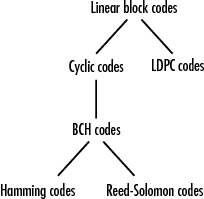
\includegraphics[scale=1]{figuras/blockcodes.png}
      \caption{Uma classifica��o para c�digos de blocos \cite{MathWorks:2010}}
      \label{fig4:cbc}
    \end{figure} 

\vspace{2cm}

Um c�digo C � linear se v e w s�o palavras c�digo distintas de um c�digo C, ent�o v+w � tamb�m uma palavra c�digo de C. Um c�digo linear cont�m a palavra c�digo zero, pois $v + v = 0$. Opera��o simples de decodifica��o, pouca mem�ria e m�todos simples para determina��o de padr�es de erros s�o algumas das vantagens de c�digos lineares.

Um c�digo C � chamado de c�clico se o deslocamento c�clico (\emph{shift}) de qualquer palavra c�digo gera uma nova palavra c�digo. Por exemplo, $C1 = \{000, 110, 101, 011\}$   � um c�digo c�clico. $C2 = \{000, 100, 011, 111\}$ n�o � um c�digo c�clico.

\subsection{C�digos Convolacionais}

P. Elias introduziu c�digos convolucionais em 1955. Um c�digo convulacional � um dispositivo com mem�ria. Apesar de aceitar uma mensagem de entrada de tamanho fixo e produzir uma sa�da codificada, seus c�lculos n�o dependem somente da entrada atual, mas tamb�m das entradas e sa�das anteriores.

Um codificador para um c�digo convolucional tamb�m aceita blocos de $k$ bits da sequ�ncia de dados $u$ e gera uma sequ�ncia de sa�da $v$ de $n$ \emph{bits} chamada \emph{codeword} ou palavra c�digo. Cada bloco da palavra c�digo n�o depende apenas dos $k$ bits do bloco da sequ�ncia de dados correspondente, mas tamb�m de $M$ blocos anteriores. Dizemos que o codificador tem mem�ria de ordem $M$, onde $M$ � o n�mero de registradores de mem�ria. Esse conjunto de blocos de $k$ bits, o codificador das palavras c�digo de tamanho $n$ e de mem�ria de ordem $M$ � chamado de ($n$, $k$, $M$) c�digo convolucional. $R = \frac{k}{n}$  � a taxa de codifica��o. Como o codificador tem mem�ria, ele pode ser implementado como circuito l�gico sequ�ncial \cite{Lin:1983}.

Em um c�digo convolucional, os $n - k$ bits redundantes, que provem � codifica��o a capacidade de tratar os ru�dos do canal, podem ser adicionados quando $k < n$. Para uma mesma taxa de codifica��o $R$, pode-se adicionar redund�ncia, aumentando a ordem da mem�ria $M$ do codificador. Como usar a mem�ria para obter uma transmiss�o confi�vel sob um canal com ru�do � o principal problema do projeto do codificador.

C�digos convolucionais podem ser usados para melhorar o desempenho da comunica��o por r�dio e sat�lites. C�digos convolucionais s�o utilizados nas tecnologias CDMA (\emph{Code division multiple access}) e GSM (\emph{Global System for Mobile Communications}) para telefones celulares, \emph{dial-up modems}, sat�lites, \emph{NASA's Deep Space Network} deep-space communications e na rede WLAN Wi-Fi IEEE 802.11.

\vspace{1cm}

Existem v�rios algoritmos de codifica��o por apagamento \cite{Byers:1998, Kubiatowicz:2000}. Alguns dos mais utilizados s�o c�digos Reed-Solomon (RS), c�digos Low-Density Parity-Check (LDPC) e c�digos Tornado \cite{Mitzenmacher:2004} \cite{RTAD:2007}.

Segundo \cite{Woitaszek:2007}, para sistemas de armazenamento, a codifica��o por apagamento baseada em opera��es simples, tais como XOR RAID e c�digos Tornado,  s�o prefer�veis. Apesar de que um mecanismo externo deva ser utilizado para detectar erros, as opera��es de XOR podem ser realizadas rapidamente e resultar em alto \emph{throughput} das opera��es de codifica��o e decodifica��o.

\subsection{Caracter�sticas de C�digos de Blocos}


A dist�ncia de Hamming (dH) entre duas palavras c�digo $v_i$ e $v_j$  � o n�mero de \emph{bits} que s�o diferentes nessas duas palavras.

Segundo \cite{AF:2010}, as principais caracter�sticas de c�digos de blocos s�o:

\begin{description}
   \item [taxa de codifica��o] $R = \frac{k}{n}$ � a medida da efici�ncia do c�digo, pois � o quociente do n�mero de \emph{bits} da palavra de dados sobre o n�mero de \emph{bits} total da palavra transmitida
   \item [dist�ncia m�nima] $(d_{min})$ � a menor dist�ncia de Hamming entre duas quaisquer palavras do c�digo; ela depende do n�mero de \emph{bits} redundantes $q = n - k$, tal que  $(d_{min} \leq q + 1)$
   \item [capacidade de detec��o] detecta at� $l$ erros, onde $l \leq d_{min} - 1$
   \item [capacidade de corre��o] corrige os erros at� $t$ erros, onde $ t \leq \lfloor \frac{d_{min} - 1}{2} \rfloor$
   \item [capacidade de detec��o e corre��o] detecta at� $l$ erros e corrige os erros at� $t$ erros, onde $d_{min} \geq l + t + 1$ e $l > t$
\end{description}

Um c�digo com $d_{min} = 1$ n�o tem capacidade de detectar erros.

\subsection{C�digos de Blocos Lineares}

\subsubsection{C�digos Reed-Solomon}

S�o c�digos de blocos, lineares e c�clicos.

Definition. A Reed-Solomon (or RS) code over GF(q) is a BCH (BOSE-CHAUDHURI-HOCQUENGHEM) code of length N = q - 1. Of course q is never 2. Thus the length is the number of nonzero elements in the ground field. We shall use N , K and D to denote the length, dimension, and minimum distance (using capital letters to distinguish them from the parameters of the binary codes which will be constructed later). RS codes are important in concatenated codes and burst correction.

Em \cite{Plank:1997}, o autor apresenta uma especifica��o completa do problema e do algoritmo da codifica��o e detalhes de sua implementa��o. O modelo estudado � formado por $n$ dispositivos de armazenamento  $D_1, D_2, ..., D_n$ (\emph{data devices}) e outros $m$ dispositivos de armazenamento  $C_1, C_2, ..., C_m$ (\emph{checksum devices}). O conte�do de cada um dos $m$ \emph{checksum devices} � calculado a partir do conte�do dos $n$ \emph{data devices}. O objetivo do c�lculo dos $C_i$ para $1 \leq i \leq m$ � tal que para quaisquer $m$ dispositivos que falhem dos $D_1, D_2, ..., D_n, C_1, C_2, ..., C_m$, o conte�do dos dispositivos que falharam possa ser reconstitu�do a partir dos dispositivos que n�o falharam.

Segundo \cite{Almeida:2007}, c�digos RS s�o particularmente �teis para corre��o de erros em rajada (seq��ncia s�mbolos consecutivos, nenhum desses recebidos corretamente, chamados \emph{burst errors}). Tamb�m podem ser usados eficientemente em canais onde o conjunto de s�mbolos de entrada � consideravelmente grande.

Uma implementa��o de biblioteca em C/C++ para o algoritmo RS foi apresentada em \cite{Plank:2007}.

O sistema de armazenamento OceanStore \cite{Kubiatowicz:2000} e o protocolo BitTorrent (aplica��o da camada de rede da internet) usam uma codifica��o RS.

\subsubsection{C�digos RAID}

\emph{Redundant Arrays of Inexpensive [Independent] Disks} (RAID) � uma classe de c�digos RS. RAID � um m�todo para prover toler�ncia a falhas ou alto desempenho em sistemas de armazenagem utilizando para isso uma codifica��o de corre��o de erros ou paridade. RAID foi introduzido por D. A. Patterson na Universidade da California, Berkeley (UC Berkeley) em 1988 \cite{Patterson:1988}.

S�o conceitos b�sicos \cite{Vadala:2002}:

\begin{description}

   \item [data striping] � uma t�cnica para segmentar dados sequ�nciais, como um arquivo, de maneira que o acesso a segmentos sequ�nciais seja feito por diferentes dispositivos de armazenamento. Esta t�cnica � �til quando se quer processar mais rapidamente os pedidos de acesso a dados que os dispositivos de armazenamento permitem. Diferentes segmentos de dados s�o mantidos em diferentes dispositivos de armazenamento. A falha de um dos dispositivos torna toda a sequ�ncia de dados indispon�vel. Essa desvantagem � superada pelo armazenamento de informa��es redundantes (custo de armazenamento extra), como a paridade, com o objetivo de corre��o de erros. As configura��es de RAID que utilizam paridade s�o RAID-2, RAID-3, RAID-4, RAID-5 e RAID-6 \cite{DS:2010}.

   \item [stripe] s�o segmentos consecutivos ou faixas que s�o escritos sequencialmente atrav�s de cada um dos discos de um \emph{array} ou conjunto. Cada segmento tem um tamanho definido em blocos.

\end{description}

\vspace{1cm}

{\bf RAID 2}

\vspace{0.5cm}

Esta configura��o divide os dados a nivel de \emph{bit} e usa c�digos Hamming para corre��o de erros. Por exemplo, o c�digo Hamming(7,4) (quatro \emph{bits} de dados e tres \emph{bits} de paridade) permite usar 7 discos em RAID 2, sendo 4 usados para armazenar dados e 3 usados para corre��o de erros. Esta codifica��o tornou-se padr�o para \emph{hard drives} e tornou-se desnecess�ria, assim deixou de ser vantajosa.

\vspace{1cm}

{\bf RAID 3}

\vspace{0.5cm}

Esta configura��o divide os dados a nivel de \emph{byte} com um disco apenas para paridade. Isto requer que todos os discos operem em \emph{lockstep} (rota��o de todos os discos em sincronismo). Assim como RAID-2, tornou-se obsoleta.

\vspace{1cm}

{\bf RAID 4}

\vspace{0.5cm}

Esta configura��o divide os dados a nivel de bloco com um disco apenas para paridade. Se o controlador de disco permitir, um conjunto RAID 4 pode atender v�rias solicita��es de leitura ao mesmo tempo. Todos os \emph{bits} de paridade est�o em um �nico disco, o que pode se tornar um gargalo. RAID-5 substituiu esta configura��o.

\vspace{1cm}

{\bf RAID 5}

\vspace{0.5cm}

Esta configura��o divide os dados a nivel de bloco com um �nico bloco de paridade por \emph{stripe} e os blocos de paridade ficam distribu�dos por todos os discos. Esta configura��o privilegia a leitura. Uma s�ndrome � computada para permitir a perda de uma unidade. Essa s�ndrome P pode ser um simples XOR de dados pelos \emph{stripes}.

\vspace{1cm}

{\bf RAID 6}

\vspace{0.5cm}

Esta configura��o divide os dados a nivel de bloco com dois blocos de paridade por \emph{stripe} e os blocos de paridade distribu�dos por todos os discos. Duas s�ndromes diferentes precisam ser computadas para permitir a perda de quaisquer duas unidades. Uma delas, P pode ser um simples XOR de dados pelos \emph{stripes}, como em RAID 5. A outra, Q pode ser um XOR de um \emph{linear feedback shift register} de cada \emph{stripe}.

Passo 0: n� 0 cria palavra c�digo em blocos b1, b2, b3, ..., bk

Passo 1: n� 0 cria b1 e o envia para os n� 1 e n� 2

Passo 2: n� 0 cria b2 e o envia para os n� 1 e n� 3

Passo 3: n� 0 cria b3 e o envia para os n� 1 e n� 4

Passo 4: n� 0 e n� 1 codificam b1, b2 e b3 e criam o bloco de paridade p1 = f1(b1, b2, b3) e p2 = f2(b1, b2, b3) 

\vspace{1cm}

\subsubsection{C�digos Low-Density Parity-Check e Tornado}

S�o c�digos de blocos, lineares e ac�clicos.

C�digo Low-Density Parity-Check (LPDC) �  uma codifica��o baseada em grafos regulares \cite{Gallager:1963}. C�digos LDPC s�o conhecidos tamb�m como c�digos Gallager \cite{LDPCC:2010}. Uma aplica��o dessa codifica��o � a rede \emph{wireless} WMAN WiMAX (IEEE 802.16e \emph{standard for microwave communications}) para internet m�vel \cite{wimax:2010}.

C�digos Tornado s�o uma classe de c�digos LDPC \cite{Woitaszek:2007}. Segundo \cite{Kubiatowicz:2000}, s�o mais r�pidos para codificar e decodificar e necessitam de um pouco mais de $m$ fragmentos para reconstruir a informa��o. 

Em \cite{Luby:1998}, os autores apresentam c�digos Tornado baseados em grafos irregulares. Segundo \cite{CS540:2010}, as implica��es pr�ticas desses c�digos ainda n�o foram bem estudadas.

%Na tabela~\ref{tab1:comp}, alguns sistemas que utilizam com
%codifica��o por apagamento foram comparados.

%
\begin{table}
\singlespacing

  \begin{center}
    \begin{tabular}{|p{2.5cm}||p{2cm}||p{2.7cm}||p{2.5cm}||p{3.5cm}|}
      \hline

Trabalho & Modelo & Objetivos & Codifica��o & M�tricas \\ \hline
Byers,1998 \cite{Byers:1998} & \emph{Digital Fountain} & Confiabilidade, Efici�ncia & Replica��o, c�digos Tornado e RS & tempo de codifica��o e decodifica��o de um bloco \emph{bandwidth}, perda de pacotes\\ \hline

Weatherspoon, 2002 \cite{Weatherspoon:2002:01} & Arquivador central, n�s & Disponibilidade & Replica��o, Codifica��o por Apagamento & tempo m�dio entre falhas, \emph{overhead} de armazenamento, tempo de verifica��o do bloco \\ \hline

Camargo, 2009 \cite{Camargo:2009} & OppStore & Confiabilidade, Disponibilidade & Replica��o  & \emph{bandwidth}, n�mero de mensagens trocadas \\ \hline

Fan, 2009 \cite{Fan:2009}& HDFS & Confiabilidade, Disponibilidade & Replica��o, RAID & atraso na codifica��o do bloco\\ \hline

Dabek, 2004 \cite{Dabek:2004} & DHT & Efici�ncia & Replica��o, Codifica��o por Apagamento & lat�ncia \\ \hline

Houri, 2009 \cite{Houri:2009} & \emph{Peer-to-peer} & Disponibilidade & Replica��o, Codifica��o por Apagamento & \emph{bandwidth} \\ \hline

Plank, 2009 \cite{Plank:2009} & $k$ discos de dados e $m$ discos de paridade & Efici�ncia & c�digos Tornado, RS e RAID & tempo de codifica��o de um grande arquivo de v�deo e tempo de decodifica��o de um \emph{drive} de dados\\ \hline
    \end{tabular}
\caption{Compara��o entre sistemas de codifica��o por apagamento}
\label{tab1:comp}
  \end{center}
\end{table}


%\subsection{Replica��o versus Codifica��o por Apagamento}

%Para implementar redund�ncia de dados em sistemas, s�o utilizadas v�rias t�cnicas: codifica��o por apagamento, replica��o, espelhamento, \emph{Cyclic redundancy check} (CRC), \emph{bits} de paridade, \emph{checksum}, assinatura digital \cite{EDC:2010}. Mecanismos de redund�ncia podem implementar um conjunto destas t�cnicas \cite{Fan:2009}.

%Entre as t�cnicas para implementar redund�ncia de dados, a replica��o � a mais utilizada em sistemas com o objetivo de se obter alta disponibilidade e durabilidade de dados diante de falhas de componentes destes sistemas. O motivo disto � a simplicidade na implementa��o de replica��o, mas algumas pesquisas demonstram um campo promissor para codifica��o por apagamento para armazenamento em sistemas distribu�dos.

%A principal desvantagem da replica��o � que ela requer um grande \emph{overhead} de armazenamento para pouco ganho em disponibilidade e toler�ncia a falhas. Garantir que os dados permane�am dispon�veis quando todos os $n$ dispositivos falham exige que, pelo menos, $n + 1$ c�pias existam \cite{Woitaszek:2007}. Por exemplo, o sistema Glaciar de armazenamento aumenta de 11 vezes a quantidade de dados armazenados utilizando replica��o para conseguir 0.999999\% (\emph{six nines})  de confiabilidade.

%Uma vantagem de codifica��o por apagamento seria um custo menor de armazenamento se comparado a replica��o, no caso de grande volume de dados. Outra vantagem com rela��o a replica��o foi comentada em \cite{Weatherspoon:2002:01}: para um mesmo espa�o de armazenamento, o tempo m�dio entre falhas (\emph{mean time to failure}) � maior.

%Os autores em \cite{Dabek:2004} afirmam que dados replicados permitem leituras de baixa lat�ncia, porque h� muitas op��es para a sele��o de servidores, enquanto que dados codificados reduzem o consumo de largura de banda para escritas, em detrimento do aumento da lat�ncia de leituras.



\section{Discuss�o sobre esquemas adequados de redund�ncia de dados}

Pode-se encontrar na literatura um n�mero significativo de projetos que prop�em sistemas de armazenamento distribu�do, sistemas de arquivos distribu�dos, ou sistemas de backup. Apesar da disso, nenhum esquema de redund�ncia de dados tem sido amplamente aceito para esses sistemas e nenhuma regra f�cil foi criada para se encontrar um esquema adequado de redund�ncia de dados.

Os autores em \cite{Duminoco:2009} estudaram redund�ncia de dados em sistemas \emph{peer-to-peer} para \emph{backup} e propuseram um esquema h�drido para implementar redund�ncia (replica��o e codifica��o) de dados. Em \cite{Storer:2008}, foi proposto um sistema de armazenamento de dados baseado em discos que usa dois n�veis de codifica��o. Nesses textos, encontramos uma compara��o entre alguns sistemas de armazenamento, avaliando-se algumas de suas caracter�sticas. Podemos observar que os tipos de esquema de redund�ncia de dados s�o replica��o, codifica��o por apagamento e h�brido, sendo a replica��o, a estrat�gia mais utilizada nos sistemas comparados por \cite{Duminoco:2009} e a codifica��o por apagamento, para os sistemas comparados por \cite{Storer:2008}.

Redund�ncia de dados � necess�ria para prevenir perda de dados, mas n�o � suficiente. A avalia��o de esquemas de redund�ncia � muitas vezes baseada na suposi��o de que as r�plicas falham de forma independente. Na pr�tica, as falhas n�o s�o t�o independentes, segundo \cite{Weatherspoon:2002:02,Baker:2006}. Esse trabalho n�o tratar� a independ�ncia das r�plicas.

Cada esquema de redund�ncia estabelece (i) como criar os dados redundantes e (ii) como reconstruir os dados quando houver falha. Essas duas opera��es geram custos que diferem de um esquema para outro. Esse trabalho comentar� os mais amplamente usados esquemas de redund�ncia: replica��o e c�digos corretores de erros.

\subsection{Esquemas de redund�ncia de dados para sistema de armazenamento}

Esquemas de redund�ncia de dados s�o utilizados em sistemas de armazenamento (exemplo: sistemas RAID) para prover disponibilidade, toler�ncia a falhas e durabilidade de dados e em sistemas de comunica��o (exemplo, sistemas \emph{peer-to-peer}) para prover uma entrega confi�vel e segura de dados.

Replica��o � o esquema de redund�ncia mais simples. A maioria dos sistemas, que utiliza redund�ncia de dados, � baseada em replica��o, mas esse esquema consume mais armazenamento que a codifica��o por apagamento.

A replica��o � usada no Google File System \cite{Ghemawat:2003} (GFS) e no Hadoop Distributed File System \cite{Hadoop:2010} (HDFS), sistemas de arquivos distribu�dos que apresentam caracter�sticas semelhantes. Um \emph{cluster} do GFS ou do HDFS � formado por um �nico servidor, master (GFS) ou namenode (HDFS), que mant�m os metadados e muitos servidores de dados, os chunkservers (GFS) ou os datanodes (HDFS) e � acessado por v�rios clientes. Os arquivos de dados s�o armazenados nos chunkservers (GFS) ou datanodes (HDFS) e particionados em blocos de igual tamanho. Ambos, GFS e HDFS foram projetados para aplica��es que processam grande volume de dados. 

Seus projetos consideram \emph{clusters} de (\emph{commodity hardware}), uma vers�o do \emph{kernel} linux como sistema operacional para as m�quinas e uma arquitetura de rede com dois n�veis: v�rios \emph{racks} interligados por um comutador e cada \emph{rack} � formado por v�rias m�quinas e seus discos, estes tamb�m interligados por um comutador. A estrat�gia de inser��o de dados cria r�plicas em \emph{racks} distintos do \emph{rack} onde est� a 1$^a$ r�plica, assim, falhas que comprometam um \emph{rack} n�o provocam a indisponibilidade de dados. Os arquivos de dados s�o alterados por concatena��es ao inv�s de sobrescrever dados existentes. Ap�s a cria��o, os arquivos de dados s�o usados apenas para leitura e esta leitura ocorre sequencialmente. As APIs do cliente fornecidas pelo GFS e pelo HDFS suportam opera��es de cria��o, leitura, escrita, remo��o, mas n�o implementam a interface POSIX.

O Farsite, que utiliza apenas replica��o, � um sistema de arquivos distribu�dos, particionados em namespaces, explorando os desktops presentes dentro da Microsoft. Ceph \footnote{http://ceph.newdream.net/} � um sistema de arquivos \emph{open source} (existe m�dulo em desenvolvimento que permite us�-lo como armazenamento para uma inst�ncia do Hadoop) e tamb�m utiliza apenas replica��o.



%\section{Hadoop}

Atualmente, o Google � uma empresa de consulta e publicidade e � capaz de fornecer os seus servi�os devido a investimentos em armazenamento distribu�do em larga escala e a capacidade de processamento, estes desenvolvidos \emph{in-house}.

Essa capacidade � fornecida por um grande n�mero de PCs, pelo Google File System (GFS), um sistema de arquivos redundantes em \emph{cluster}, pelo sistema operacional GNU/Linux e pelo MapReduce, um \emph{middleware} de processamento paralelo de dados.

Em 2004, um artigo~\cite{Dean:2004}, que foi publicado por
profissionais da Google, prop�s o MapReduce. Em 2006, estes
profissionais, juntamente com Doug Cutting do Yahoo!, formaram um
sub-projeto do Apache Lucene\footnote{http://www.apache.org} que foi
chamado Hadoop\footnote{http://hadoop.apache.org/}.

Mais recentemente, o projeto Apache Hadoop tem desenvolvido uma
reimplementa��o de partes do GFS e MapReduce e muitos grupos da
comunidade de software livre posteriormente abra�aram essa tecnologia,
permitindo-lhes fazer coisas que eles n�o poderiam fazer em m�quinas
individuais. O Hadoop est� dispon�vel em c�digo fonte sob
licenciamento Apache \emph{license} (compat�vel com GPL).

O Hadoop � um \emph{framework} para executar aplica��es em
armazenamento distribu�do de grande volume de dados que pode ser
constru�do com \emph{commodity hardware}, que � facilmente acess�vel e
dispon�vel.  O Hadoop n�o � um \emph{framework} can�nico. Ele foi
projetado para aplica��es que atualizam dados da seguinte forma: uma
escrita e muitas leituras, atrav�s de acessos por \emph{batch}, com
tamanho da ordem de petabytes, organizados de forma n�o estruturada,
com esquema din�mico e integridade baixa.  Uma lista de aplica��es e
organiza��es que usam o Hadoop pode ser encontrada em
\cite{HadoopWiki:2010}.

Em poucas palavras, o Hadoop disponibiliza um armazenamento
compartilhado (HDFS) e um sistema de an�lise (MapReduce) que comp�em o
seu \emph{kernel}.

\subsection{MapReduce}

O MapReduce utiliza algoritmos de ordena��o para reconstruir sua base de dados.  Um bom uso para o MapReduce s�o aplica��es cujos dados s�o escritos uma vez e lidos muitas vezes. S�o dados n�o estruturados como texto ou imagens. O MapReduce tenta colocar esses dados no n� onde s�o feitas as computa��es, desta forma, o acesso aos dados � r�pido, pois � local \cite{White:2009}.

O MapReduce pode resolver problemas gen�ricos, cujos dados podem ser divididos em matrizes de dados, para cada matriz a mesma computa��o necess�ria (sub-problema) e n�o existe necessidade de comunica��o entre as tarefas (sub-problemas). A execu��o de um t�pico \emph{job} do MapReduce pode ser assim descrita:

\begin{itemize}
    \item Itera��o sobre um n�mero grande de registros
    \item Map extrai algo de cada registro (chave, valor)
    \item Rearranjo (\emph{shuffle}) e ordena��o de resultados intermedi�rios por (chave, valor)
    \item Reduce agrega os resultados intermedi�rios
    \item Gera��o da sa�da
\end{itemize}

Um programas para execu��o no HFS/MapReduce que podem ser escritos em v�rias linguagens como Java, Ruby, Python e C++.


\subsection{Arquitetura do Hadoop \emph{Distributed File System}}

Um \emph{cluster} do HDFS � composto por um �nico NameNode, um
servidor-mestre que gerencia o sistema de arquivos e controla o acesso
aos arquivos de clientes. H� uma s�rie de DataNodes, geralmente um por
n� do \emph{cluster}, que gerenciam o armazenamento anexado ao n� em
que s�o executados. A Figura~\ref{fig6:hfs} mostra o NameNode e os
DataNodes.

Uma t�pica arquitetura de rede em dois n�veis para um \emph{cluster}
Hadoop � constru�da por v�rios \emph{racks} interligados por um
comutador como mostra a Figura~\ref{fig5:hc}. Cada \emph{rack} por sua
vez � formado por v�rios n�s (m�quinas) e seus discos, estes tamb�m
interligados por um comutador.

    \begin{figure}[h]
      \centering
      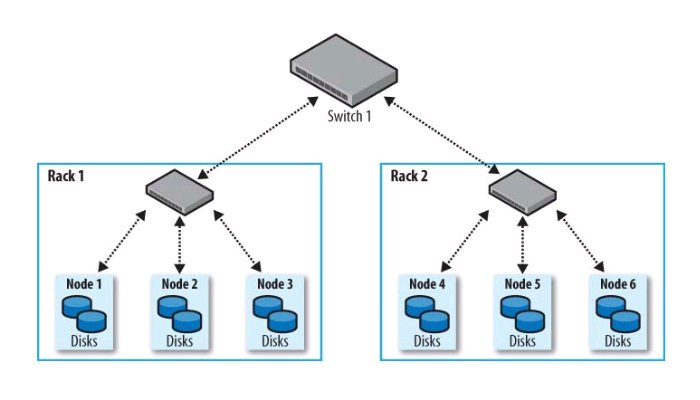
\includegraphics[scale=0.6]{figuras/hadoop-cluster.jpg}
      \caption{Arquitetura de rede em dois n�veis para um cluster Hadoop~\cite{Hadoop:2010}}
      \label{fig5:hc}
    \end{figure} 

O NameNode executa opera��es no sistema de arquivos, como \emph{open}, \emph{close}, \emph{rename} de arquivos e de diret�rios.

HDFS disponibiliza espa�o para sistema de arquivos e permite que os
dados do usu�rio sejam armazenados em arquivos. Internamente, um
arquivo � dividido em um ou mais blocos e esses blocos s�o armazenados
em um conjunto de DataNodes. A Figura~\ref{fig7:hfs} mostra DataNodes
e seus blocos. O tamanho \emph{default} de cada bloco � 64MB.

    \begin{figure}[htbp]
      \centering
      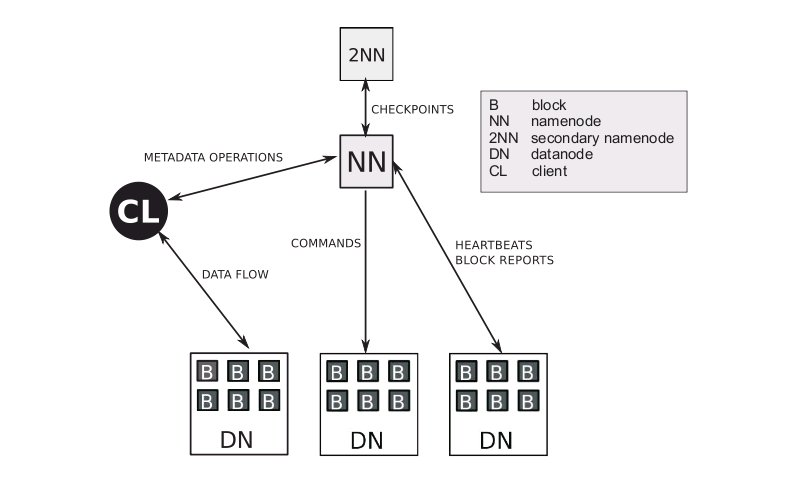
\includegraphics[scale=.6]{figuras/HDFS-arquitetura-2.jpg}
      \caption{Arquitetura do HDFS \cite{TR-IC-10-24}}
      \label{fig6:hfs}
    \end{figure} 

Os DataNodes respondem aos pedidos de leitura e escrita de clientes do
sistema de arquivos e tamb�m executam a cria��o, elimina��o e
replica��o de blocos sob instru��o do NameNode. O n�mero de r�plicas �
geralmente 3. A 1$^a$ r�plica fica local, no mesmo n� do c�digo do
cliente. A 2$^a$ r�plica fica em um n� em outro \emph{rack} e a 3$^a$
r�plica fica nesse �ltimo \emph{rack} em outro n�. As 2$^a$ e 3$^a$
r�plicas n�o s�o locais ao bloco replicado.

O NameNode e DataNode s�o partes do \emph{software} projetado para
rodar em \emph{commodity hardware}. Essas m�quinas normalmente
executam um sistema operacional GNU/Linux.

HDFS � constru�do usando a linguagem Java. Qualquer m�quina que suporte
Java pode executar o NameNode ou o DataNode \cite{Hadoop:2010}.

\begin{figure}[h]
  \centering
  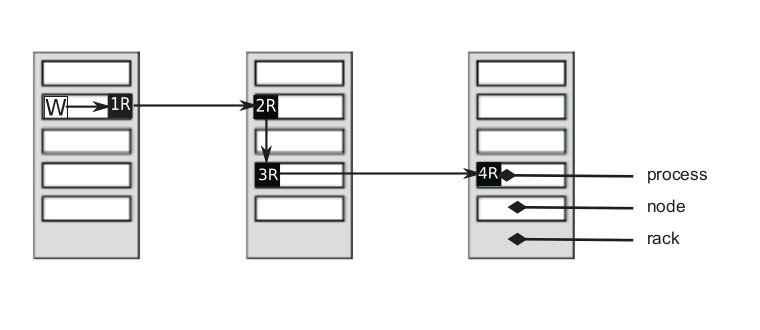
\includegraphics[scale=.5]{figuras/HDFS-arquitetura-replicacao-2.jpg}
  \caption{Arquitetura do HFS - Datanodes e Blocos \cite{White:2009}}
  \label{fig7:hfs}
\end{figure} 

Os protocolos do HDFS usam o protocolo TCP/IP. O cliente fala o
protocolo ClientProtocol com o NameNode atrav�s de uma porta. Os
DataNodes falam o protocolo DataNodeProtocol com o NameNode. Esses
protocolos executam uma \emph{Remote Procedure Call} (RPC). O NameNode
n�o inicia chamadas RPCs. Ele responde a chamadas RPCs feitas pelo
DataNodes e pelos clientes.


\subsection{Codifica��o por apagamento}

Existe uma nova caracter�stica proposta em 2009 para implementa��o de
uma camada de codifica��o por apagamento no Hadoop utilizando
RAID~\cite{HDFS-503:2010} e uma mais recente utilizando c�digos
RS~\cite{MR-1969:2010}.

A vers�o atual do Hadoop utiliza apenas a t�cnica de replica��o
\cite{White:2009} para obter disponibilidade e confiabilidade de
dados. A inclus�o da codifica��o por apagamento ser� feita com o
objetivo de reduzir o tamanho do armazenamento do HDFS.


%\input{secoes/proposta}

%\input{secoes/plano}

%\singlespacing
\setstretch{1.5}
\bibliography{referencias/ref-dissertacao}

\printindex

\end{document}
